\newpage
\chapter{Коэффициенты отражения и прохождения в одномерных задачах. Примеры}

\par 
\begin{wrapfigure}[9]{l}{0.25\linewidth} 
\vspace{-2ex}
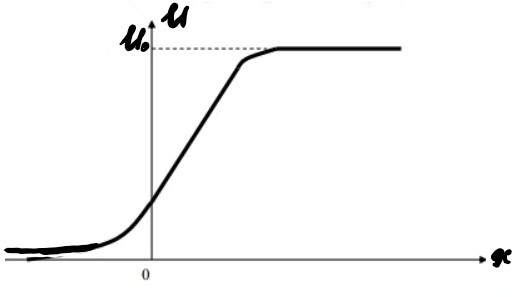
\includegraphics[width=1\linewidth]{pictures/21.1.jpg}
\caption{Вид рассматриваемого потенциала}
\end{wrapfigure}
\par При очень больших значениях $x\rightarrow \infty$ волновая функция будет выглядеть следующим образом (из граничных условий выбрали нулевой второй коэффициент) $\psi = A e^{ik_2x}$, где $k_2=\frac{1}{\hbar}\sqrt{2m(E-U_0)}$.
\par При отрицательных больших значениях $x\rightarrow -\infty$ получим с выбранным первым единичным коэффициентом: $\psi = e^{ik_1x} +B e^{-ik_1x} $, где $k_1 = \frac{1}{\hbar} \sqrt{2mE}$.
\par Плотность потока в падающей волне $k_1$, в отраженной $k_1|B|^2$, в прошедшей $k_2|A|^2$. Коэффициент прохождения $T=\frac{k_2}{k_1}|A|^2$, коэффициент отражения $R=B^2=1-T$.
\par Если дано произвольное стационарное состояние с E>$U_0$, зададим волновую функцию на $x=-\infty$ и $x=\infty$ соотвественно:
$$\psi=A_1 e^{ik_1x}+B_1 e^{-ik_1x} \text{, и }\psi=A_2 e^{ik_2x}+B_2 e^{-ik_2x}$$
\par Причем коэффициенты линейно связаны, т.к. представленные функции - это решение одного линейного лифференциального уравнения: $A_2=\alpha A_1+\beta B_1 $, где $\alpha $ и $\beta$ зависят от вида потенциала.
\par Знаем, что если $\psi$ - решение, то и $\psi^*$ тоже является решением (грубо говоря, мы инвертируем время $ t \rightarrow - t$):
$$\psi^*=A^*_1 e^{-ik_1x}+B^*_1 e^{ik_1x} \text{ при x} \rightarrow-\infty \text{, и при x} \rightarrow\infty\textit{ } \psi=A^*_2 e^{-ik_2x}+B^*_2 e^{ik_2x}$$
\par Роль $A_2$ теперь играет $B^*_2$, а т.к. это тоже решение, то можем определить связь коэффициентов:
$$B^*_2 = \alpha B^*_1 + \beta A^*_1 \textit{ или } B_2 = \alpha^* B_1 + \beta^* A_1$$
\par Постоянство потока даст $ k_1 (|A_1|^2 - |B_1|^2)=k_2 (|A_2|^2 - |B_2|^2)$ или $|\alpha|^2-|\beta|^2= \frac{k_1}{k_2}$.
\par Коэффициенты отражения совпадают при движении по и против оси Ох. Покажем это. Пусть $B_2=0$, тогда $\frac{B_1}{A_1}=-\frac{\beta^*}{\alpha^*}$ и коэффициент отражения слева $R_1 =|\frac{B_1}{A_1}|^2 = |\frac{\beta}{\alpha}|^2$. Теперь $A_1=0$ и $\frac{A_2}{B_2}=\frac{\beta}{\alpha^*}$, значит, коэффициент отражения справа $R_2 =|\frac{A_2}{B_2}|^2 = |\frac{\beta}{\alpha}|^2$, что мы и получали при вычислении коэффициента отражения слева.